\section{Introduction}
Software is the basis of all applications. Based on the performance and programmability constraints of the
system, the software engineer is tasked with determining the best implementation platform
to get a project to market. To accomplish this task, the software engineer is aided by both
programming techniques and a variety of hardware processing platforms.

\par On the programming side, previous decades yielded advances in object-oriented
programming for code reuse and parallel computing paradigms for boosting algorithm
performance. The advancements in programming languages, frameworks, and tools
allowed the software engineer to quickly prototype and test different approaches to solve
a particular problem.

\par Although the interest in the parallel and concurrent execution of software
programs is not new, the renewed and increased interest is aided by certain trends in
processor and application-specific integrated circuit (ASIC) design. There are two crucial 
factors for getting more performance out of a software algorithm  with the use of a
custom-integrated circuit or an FPGA:
\begin{itemize}
  \item Cost to fabricate the circuit
  \item Time to translate the algorithm into hardware 
\end{itemize}

Despite advancements in fabrication process node technology that have yielded significant
improvements in power consumption, computational throughput, and logic density, the
cost to fabricate a custom-integrated circuit or ASIC for an application is still high. At each
processing node, the cost of fabrication continues to increase to the point where this
approach is only economically viable for applications that ship in the range of millions of
units.

\par The second option is to use an FPGA, which addresses the cost issues inherent in ASIC
fabrication. FPGAs allow the designer to create a custom circuit implementation of an
algorithm using an off-the-shelf component composed of basic programmable logic
elements. This platform offers the power consumption savings and performance benefits of
smaller fabrication nodes without incurring the cost and complexity of an ASIC
development effort. Similar to an ASIC, an algorithm implemented in an FPGA benefits from
the inherent parallel nature of a custom circuit.

\clearpage
\subsection{Programming Model}

The programming model of a hardware platform is one of the driving factors behind its adoption. Software algorithms are typically captured in C/C++ or some other high-level
language, which abstracts the details of the computing platform. These languages allow for
quick iteration, incremental improvements, and code portability, which are critical to the
software engineer.

\par With the recent paradigm shift in the design of standard and specialized processors, both
types of processors stopped relying on clock frequency increases for program speedup and
added more processing cores per chip. Multicore processors put program parallelization at
the forefront of techniques used to boost software performance. The software engineer
must now structure algorithms in a way that leads to efficient parallelization for
performance. The techniques required in algorithm design use the same base elements of
FPGA design. The main difference between an FPGA and a processor is the programming
model.

\par Historically, the programming model of an FPGA was centered on register-transfer level
(RTL) descriptions instead of C/C++. Although this model of design capture is completely
compatible with ASIC design, it is analogous to assembly language programming in
software engineering. 

\par Both the initial and optimized versions of an application with an
FPGA platform provide significant performance when compared against the same 
stages for both standard and specialized
processors. RTL coding and an FPGA optimized application result in the highest
performance implementation. However, the development time required to arrive at this implementation is beyond the
scope of a typical software development effort. Therefore, FPGAs were traditionally used
only for those applications requiring a performance profile that could not be achieved by
any other means, such as designs with multiple processors.

\par Recent technological advances by Xilinx remove the difference in programming models
between a processor and an FPGA. Just as there are compilers from C and other high-level
languages to different processor architectures, the Xilinx Vivado High-Level Synthesis
(HLS) compiler provides the same functionality for C/C++ programs targeted to Xilinx
FPGAs.

\clearpage
\section{FPGA Architecture}   
An FPGA is a type of integrated circuit (IC) that can be programmed for different algorithms
after fabrication. Modern FPGA devices consist of up to two million logic cells that can be
configured to implement a variety of software algorithms. Although the traditional FPGA
design flow is more similar to a regular IC than a processor, an FPGA provides significant
cost advantages in comparison to an IC development effort and offers the same level of
performance in most cases. Another advantage of the FPGA when compared to the IC is its
ability to be dynamically reconfigured. This process, which is the same as loading a program
in a processor, can affect part or all of the resources available in the FPGA fabric.

\par The basic structure of an FPGA is composed of the following elements:
\begin{itemize}
  \item Look-up table (LUT): This element performs logic operations.
  \item Flip-Flop (FF): This register element stores the result of the LUT.
  \item Wires: These elements connect elements to one another.
  \item Input/Output (I/O) pads: These physically available ports get data in and out of the FPGA.
\end{itemize}

The combination of these elements results in the basic FPGA architecture shown in \figref{FPGAArch}. 
Although this structure is sufficient for the implementation of any algorithm,
the efficiency of the resulting implementation is limited in terms of computational
throughput, required resources, and achievable clock frequency.

\begin{figure}[H]
  \begin{center}
      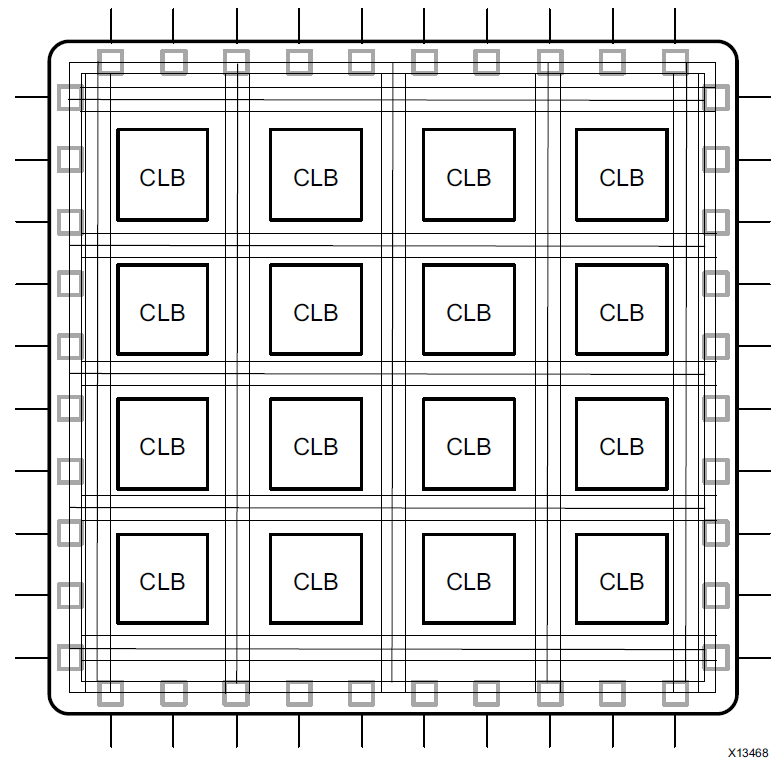
\includegraphics[width=0.75\textwidth]{images/FPGAArch.png}
      \caption{Basic FPGA Architecture}
      \label{FPGAArch}
  \end{center}
\end{figure}

\clearpage


Contemporary FPGA architectures incorporate the basic elements along with additional
computational and data storage blocks that increase the computational density and
efficiency of the device. These additional elements are:
\begin{itemize}
  \item Embedded memories for distributed data storage
  \item Phase-locked loops (PLLs) for driving the FPGA fabric at different clock rates
  \item High-speed serial transceivers
  \item Off-chip memory controllers
  \item Multiply-accumulate blocks
\end{itemize}

The combination of these elements provides the FPGA with the flexibility to implement any
software algorithm running on a processor and results in the contemporary FPGA architecture shown in \figref{ContempFPGAArch}.

\begin{figure}[H]
  \begin{center}
      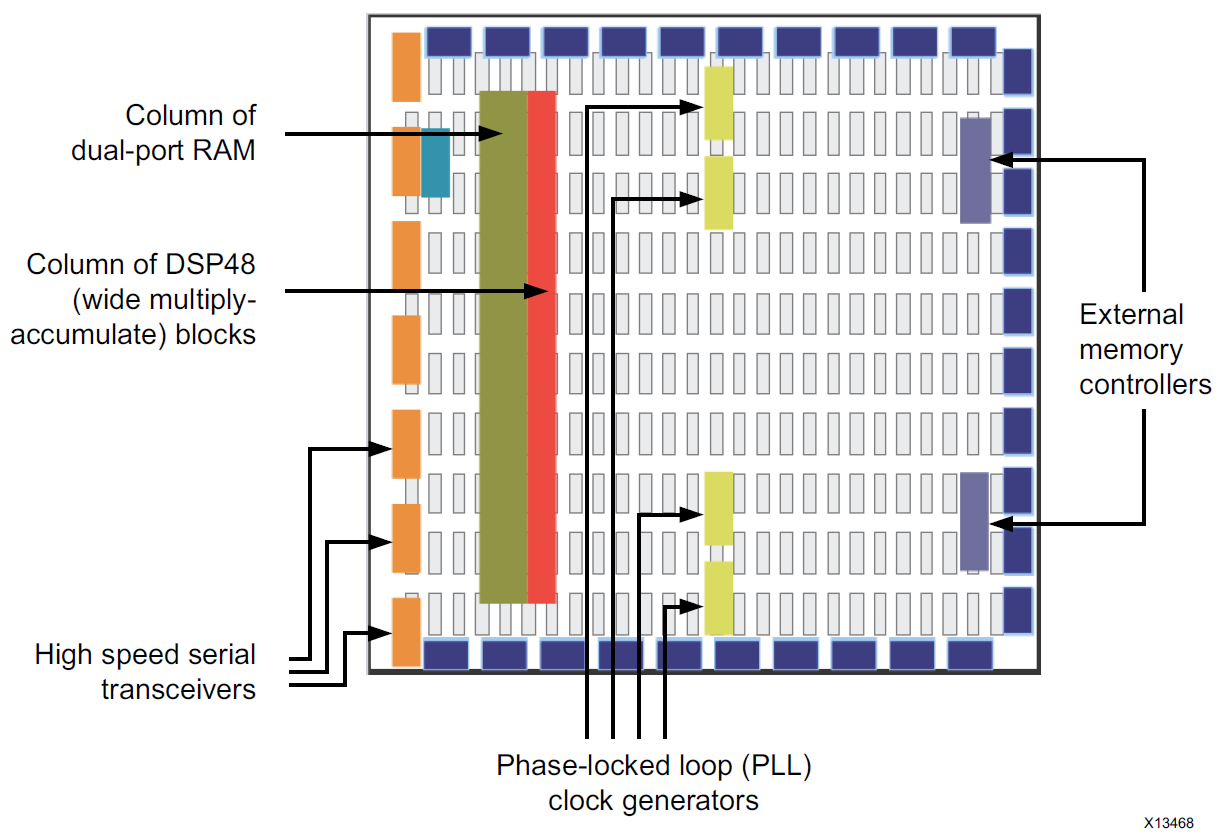
\includegraphics[width=\textwidth]{images/ContempFPGAArch.png}
      \caption{Contemporary FPGA Architecture}
      \label{ContempFPGAArch}
  \end{center}
\end{figure}

\clearpage
\subsection{Look Up Table (LUT)}
The LUT is the basic building block of an FPGA and is capable of implementing any logic
function of N Boolean variables. Essentially, this element is a truth table in which different
combinations of the inputs implement different functions to yield output values. The limit
on the size of the truth table is N, where N represents the number of inputs to the LUT. For
the general N-input LUT, the number of memory locations accessed by the table is:
\[ 2^{N} \]
which allows the table to implement the following number of functions:
\[ 2^{N^{N}} \]

\begin{highlight}
  Note: A typical value for N in Xilinx FPGA devices is 6.  
\end{highlight}

The hardware implementation of a LUT can be thought of as a collection of memory cells
connected to a set of multiplexers. The inputs to the LUT act as selector bits on the
multiplexer to select the result at a given point in time. It is important to keep this
representation in mind, because a LUT can be used as both a function compute engine and
a data storage element. \figref{LUT} shows this functional representation of the LUT.

\begin{figure}[H]
  \begin{center}
      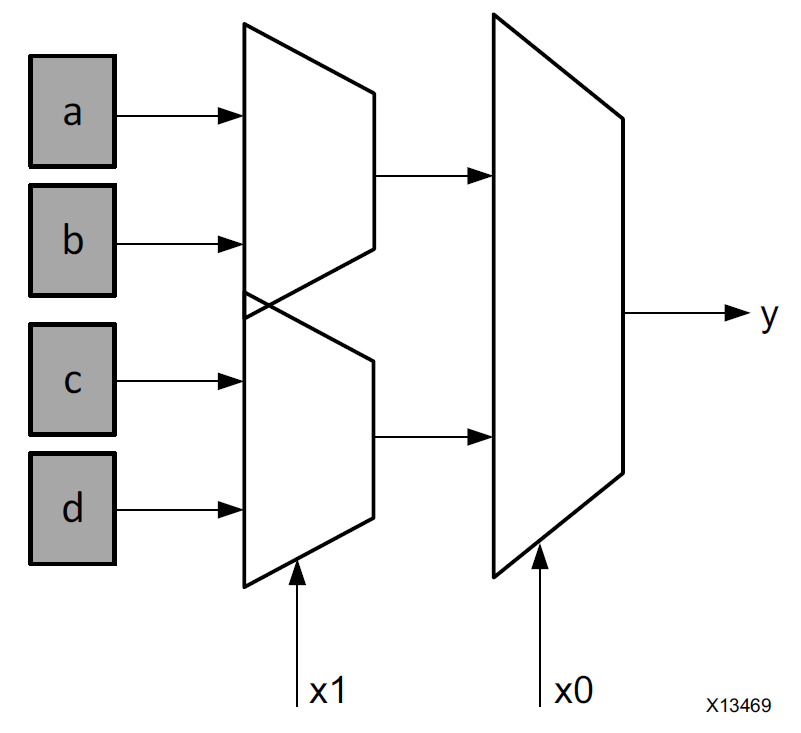
\includegraphics[width=0.6\textwidth]{images/LUT.png}
      \caption{Functional Representation of a LUT as Collection of Memory Cells}
      \label{LUT}
  \end{center}
\end{figure}

\clearpage

\subsection{Flip-Flop}

The flip-flop is the basic storage unit within the FPGA fabric. This element is always paired
with a LUT to assist in logic pipelining and data storage. The basic structure of a flip-flop
includes a data input, clock input, clock enable, reset, and data output. During normal
operation, any value at the data input port is latched and passed to the output on every
pulse of the clock. The purpose of the clock enable pin is to allow the flip-flop to hold a
specific value for more than one clock pulse. New data inputs are only latched and passed
to the data output port when both clock and clock enable are equal to one. \figref{flipflop}
shows the structure of a flip-flop.

\begin{figure}[H]
  \begin{center}
      \includegraphics[width=0.4\textwidth]{images/flipflop.png}
      \caption{Structure of a Flip-Flop}
      \label{flipflop}
  \end{center}
\end{figure}
\clearpage

\subsection{DSP Block}
The most complex computational block available in a Xilinx FPGA is the DSP block, which is
shown in \figref{dsp}. The DSP block is an arithmetic logic unit (ALU) embedded into the
fabric of the FPGA, which is composed of a chain of three different blocks. The
computational chain in the DSP is composed of an add/subtract unit connected to a
multiplier connected to a final add/subtract/accumulate engine. This chain allows a single
DSP unit to implement functions of the form:
\[ p \: =\: a*( b + d) + c\] 
or
\[ p \: +=\: a*( b + d) \] 

\begin{figure}[H]
  \begin{center}
      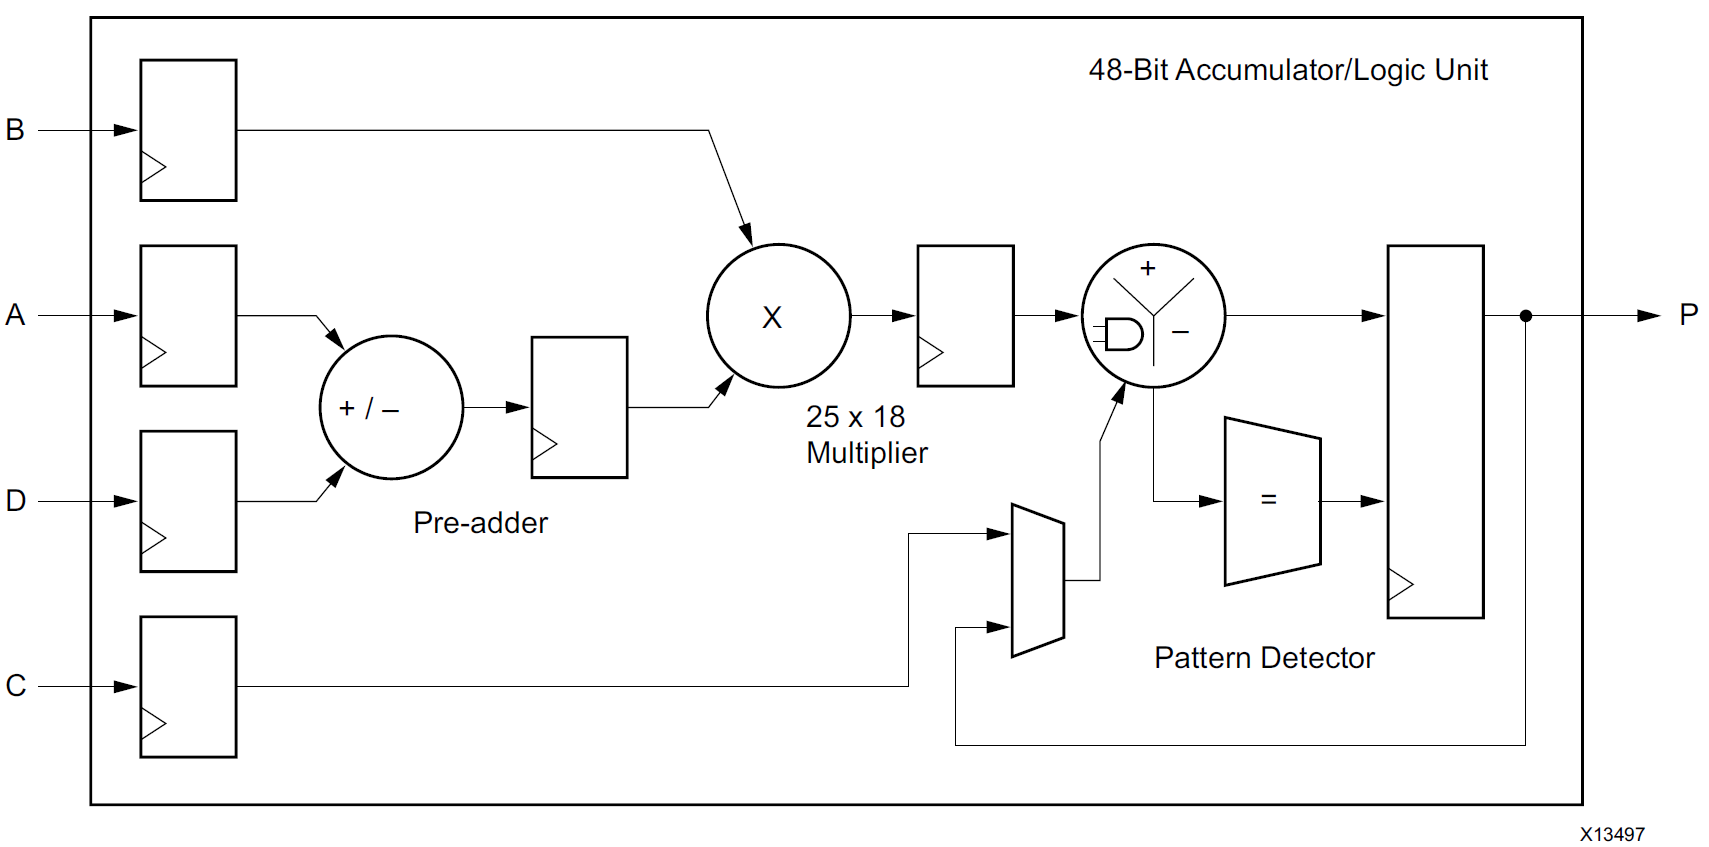
\includegraphics[width=\textwidth]{images/dsp.png}
      \caption{Structure of a DSP Block}
      \label{dsp}
  \end{center}
\end{figure}

\clearpage
\subsection{Storage Elements}
The FPGA device includes embedded memory elements that can be used as random-access memory (RAM), read-only memory (ROM), or shift registers. These elements are:

\begin{enumerate}
  \item Block RAMs (BRAMs), 
  \item UltraRAM blocks (URAMS),
  \item LUTs, and 
  \item Shift registers (SRLs).
\end{enumerate} 

\subsubsection{BRAM}
The BRAM is a dual-port RAM module instantiated into the FPGA fabric to provide on-chip storage for a relatively large set of data. The two types of BRAM memories available in a
device can hold either 18k or 36k bits. The number of these memories available is device
specific. The dual-port nature of these memories allows for parallel, same-clock-cycle
access to different locations.
In terms of how arrays are represented in C/C++ code, BRAMs can implement either a RAM
or a ROM. The only difference is when the data is written to the storage element. In a RAM configuration, the data can be read and written at any time during the runtime of the
circuit. In contrast, in a ROM configuration, data can only be read during the runtime of the
circuit. The data of the ROM is written as part of the FPGA configuration and cannot be
modified in any way.

\subsubsection{URAM}
The UltraRAM blocks are dual-port, synchronous 288 Kb RAM with a fixed configuration of
4,096 bits deep and 72 bits wide. They are available on UltraScale+ Devices and provide 8
times more storage capacity than the BRAM.

\subsubsection{LUT}
As previously discussed, the LUT is a small memory in which the contents of a truth table are
written during device configuration. Due to the flexibility of the LUT structure in Xilinx
FPGAs, these blocks can be used as 64-bit memories and are commonly referred to as
distributed memories. This is the fastest kind of memory available on the FPGA device,
because it can be instantiated in any part of the fabric that improves the performance of the
implemented circuit.

\subsubsection{Shift Register}
The shift register is a chain of registers connected to each other. The purpose of this
structure is to provide data reuse along a computational path. 


\clearpage
\section{FPGA Parallelism Versus Processor Architectures}
When compared with processor architectures, the structures that comprise the FPGA fabric
enable a high degree of parallelism in application execution. The custom processing
architecture generated by the Vivado HLS compiler for a software program presents a
different execution paradigm, which must be taken into account when deciding to port an
application from a processor to an FPGA. 

\subsection{Program Execution on a Processor}
A processor, regardless of its type, executes a program as a sequence of instructions that
translate into useful computations for the software application. This sequence of
instructions is generated by processor compiler tools, such as the GNU Compiler Collection
(GCC), which transform an algorithm expressed in C/C++ into assembly language
constructs that are native to the processor. 

\par Any assembly code can show that even a simple operation, results in multiple assembly instructions. 
The computational latency of each instruction is not equal across instruction types. 

\begin{highlight}
  IMPORTANT: The level of effort required by the software engineer in restructuring algorithms to better fit the available processor cache is not required when the same operation is implemented in an FPGA.
\end{highlight}

\subsection{Program Execution on an FPGA}
The FPGA is an inherently parallel processing fabric capable of implementing any logical
and arithmetic function that can run on a processor. The main difference is that the Vivado
HLS compiler, which is used to transform software descriptions into RTL, is not hindered by
the restrictions of a cache and a unified memory space. Every code is compiled by Vivado HLS into several LUTs required to achieve the
size of the output operand.

\begin{highlight}
  NOTE: As a general rule, 1 LUT is equivalent to 1 bit of computation.
\end{highlight}

LUTs used for a computation of a value are exclusive to that particular operation only. Unlike a
processor, where all computations share the same ALU, an FPGA implementation
instantiates independent sets of LUTs for each computation in the software algorithm. 

\par In addition to assigning unique LUT resources per computation, the FPGA differs from a
processor in both memory architecture and the cost of memory accesses. In an FPGA
implementation, the Vivado HLS compiler arranges memories into multiple storage banks
as close as possible to the point of use in the operation. This results in an instantaneous
memory bandwidth, which far exceeds the capabilities of a processor. 

\par With regard to computational throughput and memory bandwidth, the Vivado HLS
compiler exercises the capabilities of the FPGA fabric through the processes of scheduling,
pipelining, and dataflow. Although transparent to the user, these processes are integral
stages of the software compilation process that extract the best possible circuit-level
implementation of the software application.

\subsubsection{Scheduling}
Scheduling is the process of identifying the data and control dependencies between
different operations to determine when each will execute. Vivado HLS analyzes dependencies between adjacent operations as well as across time. This
allows the compiler to group operations to execute in the same clock cycle and to set up the
hardware to allow the overlap of function calls. The overlap of function call executions
removes the processor restriction that requires the current function call to fully complete
before the next function call to the same set of operations can begin. This process is called
pipelining.

\subsubsection{Pipelining}
Pipelining is a digital design technique that allows the designer to avoid data dependencies
and increase the level of parallelism in an algorithm hardware implementation. The data
dependence in the original software implementation is preserved for functional
equivalence, but the required circuit is divided into a chain of independent stages. All
stages in the chain run in parallel on the same clock cycle. The only difference is the source
of data for each stage. Each stage in the computation receives its data values from the result
computed by the preceding stage during the previous clock cycle. 

\subsubsection{Dataflow}
Dataflow is another digital design technique, which is similar in concept to pipelining. The
goal of dataflow is to express parallelism at a coarse-grain level. In terms of software
execution, this transformation applies to parallel execution of functions within a single
program. 

\par Vivado HLS extracts this level of parallelism by evaluating the interactions between different
functions of a program based on their inputs and outputs. The simplest case of parallelism
is when functions work on different data sets and do not communicate with each other. In
this case, Vivado HLS allocates FPGA logic resources for each function and then runs the blocks independently. The more complex case, which is typical in software programs, is when one function provides results for another function. This case is referred to as the consumer-producer scenario. Vivado HLS supports two use models for the consumer-producer scenario: 

\begin{itemize}
  \item In the first use
  model, the producer creates a complete data set before the consumer can start its
  operation. Parallelism is achieved by instantiating a pair of BRAM memories arranged as
  memory banks ping and pong. Each function can access only one memory bank, ping or
  pong, for the duration of a function call. When a new function call begins, the
  HLS-generated circuit switches the memory connections for both the producer and the
  consumer. This approach guarantees functional correctness but limits the level of
  achievable parallelism to across function calls.
  \item In the second use model, the consumer can start working with partial results from the
  producer, and the achievable level of parallelism is extended to include execution within a
  function call. The Vivado HLS-generated modules for both functions are connected through
  the use of a first in, first out (FIFO) memory circuit. This memory circuit, which acts as a
  queue in software programming, provides data-level synchronization between the modules.
  At any point during a function call, both hardware modules are executing their
  programming. The only exception is that the consumer module waits for some data to be
  available from the producer before beginning computation. In Vivado HLS terminology, the
  wait time of the consumer module is referred to as the interval or initiation interval (II).
\end{itemize}
\clearpage

\section{Basic Concepts of Hardware Design}

\textbf{One of the key differences between a processor and an FPGA is whether the processing
architecture is fixed.}

\par With a processor, the computation architecture is fixed, and the job of the compiler is to
determine how to best fit the software application in the available processing structures. Performance is a function of how well the application maps to the capabilities of the
processor and the number of processor instructions needed for correct execution.

\par In contrast, an FPGA is similar to a blank slate with a box of building blocks with the processing architecture not fixed. The job of the Vivado HLS compiler is to create a processing architecture from the box of building blocks that best fits the software program. The process of guiding the Vivado HLS compiler to
create the best processing architecture requires fundamental knowledge about hardware design concepts. As with processor compilers, the Vivado HLS compiler handles the
low-level details of the algorithm implementation into the FPGA logic fabric.

\subsection{Clock Frequency}

The processor clock frequency is one of the first items to consider when determining the
execution platform of a specific algorithm. A commonly used guideline is that a high clock
frequency translates into a higher performance execution rate of an algorithm. Although
this might be a good first order rule for choosing between processors, it is actually
misleading and can lead the designer to make the wrong choice when selecting between a
processor and an FPGA.

\subsubsection{Instruction execution}
The first major difference between a processor and an FPGA is how a software program is
executed. A processor is able to execute any program on a common hardware platform. This
common platform comprises the core of the processor and defines a fixed architecture onto
which all software must be fitted. The compiler, which has a built-in understanding of the
processor architecture, compiles the user software into a set of instructions. 

\par Regardless of the type of processor, standard versus specialized, the execution of an
instruction is always the same. Each instruction of the user application must go through the
following stages:
\begin{enumerate}
  \item Instruction fetch (IF)
  \item Instruction decode (ID)
  \item Execute (EXE)
  \item Memory operations (MEM)
  \item Write back (WB)
\end{enumerate}
The purpose of each stage is summarized below.
\begin{table}[H]
  \begin{tabular}{|p{0.1\linewidth} | p{0.85\linewidth}|}
  \hline
  \textbf{Stage} & \textbf{Description}                                                               \\ \hline
  IF             & Get the instruction from program memory.                                           \\ \hline
  ID             & Decode the instruction to determine the operation and the operators.             \\ \hline
  EXE            & Execute the instruction on the available hardware. In a standard processor, this means the arithmetic logic unit (ALU) or floating point unit (FPU). A specialized processor adds on fixed function accelerators to the capabilities of the standard processor at this stage of instruction processing. \\ \hline
  MEM            & Fetch data for the next instruction using memory operations.                     \\ \hline
  WB             & Write the results of the instruction either to local registers or global memory. \\ \hline
  \end{tabular}
\end{table}

Most modern processors include multiple copies of the instruction execution path and are
capable of running instructions with some degree of overlap. Because instructions in a
processor usually depend on each other, the overlap between copies of the instruction
execution hardware is not perfect. In the best of cases, only the overhead stages introduced
by using a processor can be overlapped. The EXE stages, which are responsible for
application computation, execute sequentially. The reasons for this sequential execution are
related to limited resources in the EXE stage and dependence between instructions.

\par \figref{multiProcessor} shows a processor with multiple instructions executing in a semi-parallel order.
This is the best case for a processor in which all instructions are executing as quickly as
possible. Even in this best case, the processor is limited to only one EXE stage per clock
cycle. This means that the user application moves forward by one operation per clock cycle.
Even if the compiler determined that all five EXE stages could execute in parallel, the
structure of the process would prevent it.

\begin{figure}[H]
  \begin{center}
      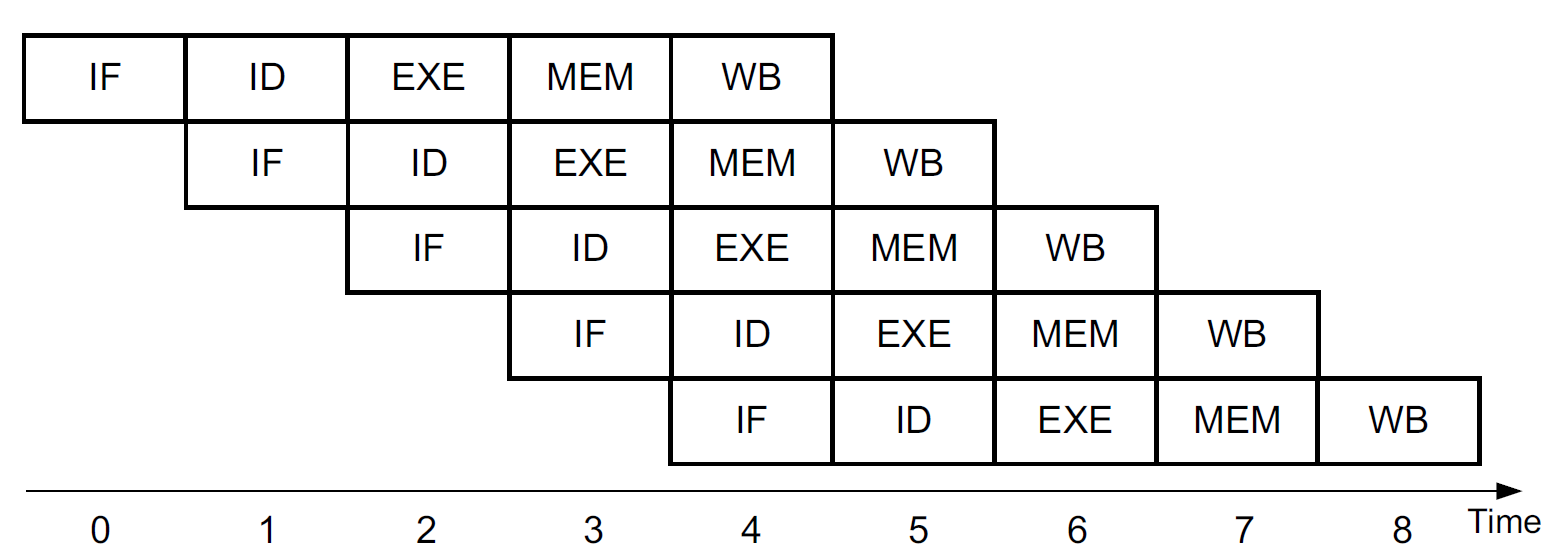
\includegraphics[width=0.8\textwidth]{images/multiProcessor.png}
      \caption{Processor with Multiple Instruction Execution Units}
      \label{multiProcessor}
  \end{center}
\end{figure}

An FPGA does not execute all software on a common computation platform. It executes a
single program at a time on a custom circuit for that program. Therefore, changing the user
application changes the circuit in the FPGA. Given this flexibility, the Vivado HLS compiler does not need to account for overhead stages
in the platform and can find ways of maximizing instruction parallelism. Working with the
same assumptions as in \figref{multiProcessor}, the execution profile of the same software in an FPGA is
shown in \figref{multiFPGA}

\begin{figure}[H]
  \begin{center}
      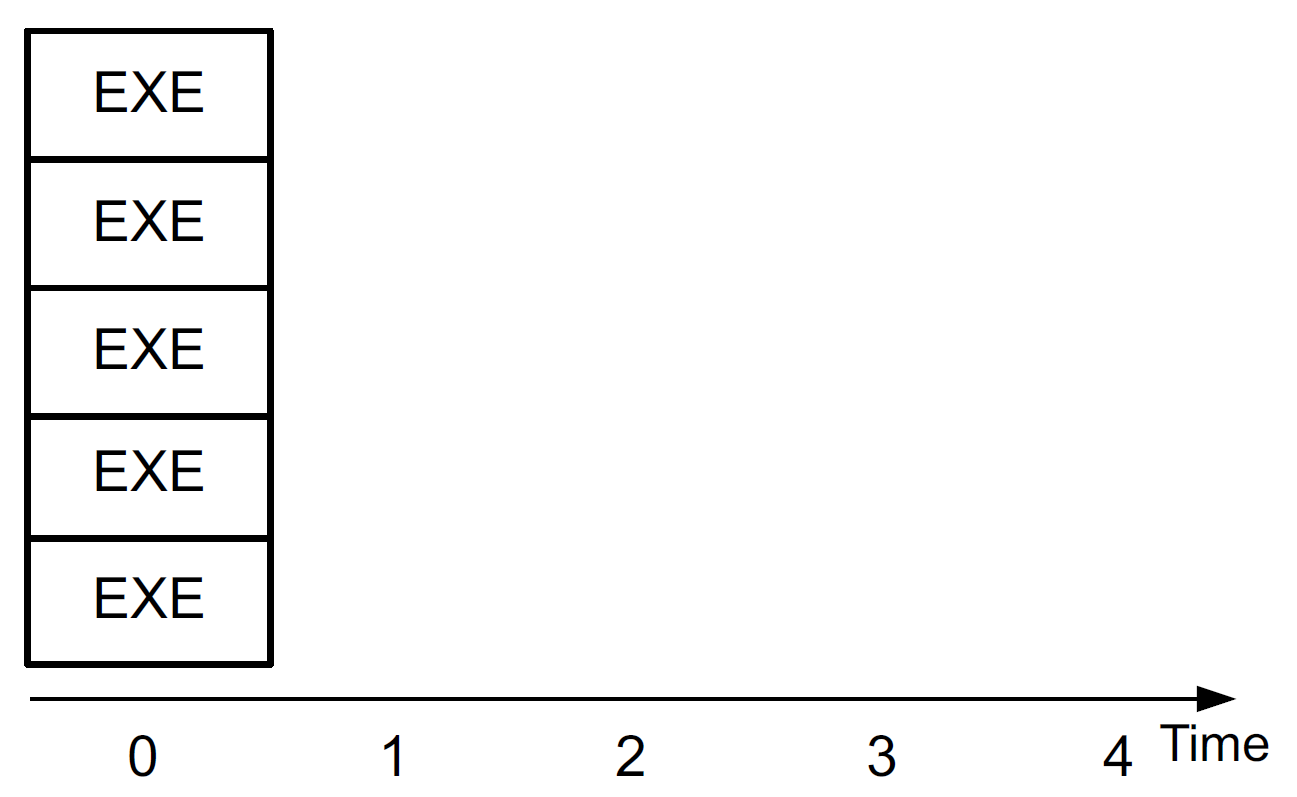
\includegraphics[width=0.6\textwidth]{images/multiFPGA.png}
      \caption{FPGA with Multiple Instruction Execution Units}
      \label{multiFPGA}
  \end{center}
\end{figure}

Based on the comparison of \figref{multiProcessor} and \figref{multiFPGA}, the FPGA has a nominal
performance advantage of 9x compared to the processor. Actual numbers are always
application specific, but FPGAs generally demonstrate at least 10x the performance of a
processor for computationally intensive applications.

\subsubsection{Power Consumption}
Another issue hidden by only focusing on the clock frequency is the power consumption of
a software program. The approximation to power consumption is given by:

\[ P = (1/2) cFV^2 \]

The relationship between power consumption and clock
frequency is supported by empirical data, which shows higher power usage in a processor
than an FPGA for the same computational workload. By creating a custom circuit per
software program, an FPGA is able to run at a lower clock frequency with maximum
parallelism between operations and without the instruction interpretation overhead found
in a processor.

\subsection{Latency and Pipelining}

\textbf{Latency} is the number of clock cycles it takes to complete an instruction or set of instructions to generate an application result value. Using the basic processor architecture, the latency of an instruction is five clock cycles. If the application has
a total of five instructions, the overall latency for this simple model is 25 clock cycles. That is, the result of the application is not available until 25 clock cycles expire. Application latency is a key performance metric in both FPGAs and processors. In both cases, the problem of latency is resolved through the use of pipelining. 

\par In a processor, pipelining means that the next instruction can be launched into execution before the
current instruction is complete. This allows the overlap of overhead stages required in
instruction set processing. By overlapping the execution of instructions, the processor achieves a latency of nine clock cycles for the five instruction application.

\par In an FPGA, the overhead cycles associated with instruction processing are not present. The
latency is measured by how many clock cycles it takes to run the EXE stage of the original
processor instruction. In the case of FPGA, the latency is one clock cycle.Parallelism also plays an important role in latency. For the full five instruction application, the FPGA latency is one clock cycle, as shown in \figref{multiFPGA}. With the one clock cycle latency of
the FPGA, it might not be clear why pipelining is advantageous. However, the reason for
pipelining in an FPGA is the same as in a processor, that is, to improve application
performance.

\par As previously explained, the FPGA is a blank slate with building blocks that must be  connected to implement an application. The Vivado HLS compiler can connect the blocks
directly or through registers. \figref{FPGAWOPipe} shows an implementation of the EXE stages without Pipelining.

\begin{figure}[H]
  \begin{center}
      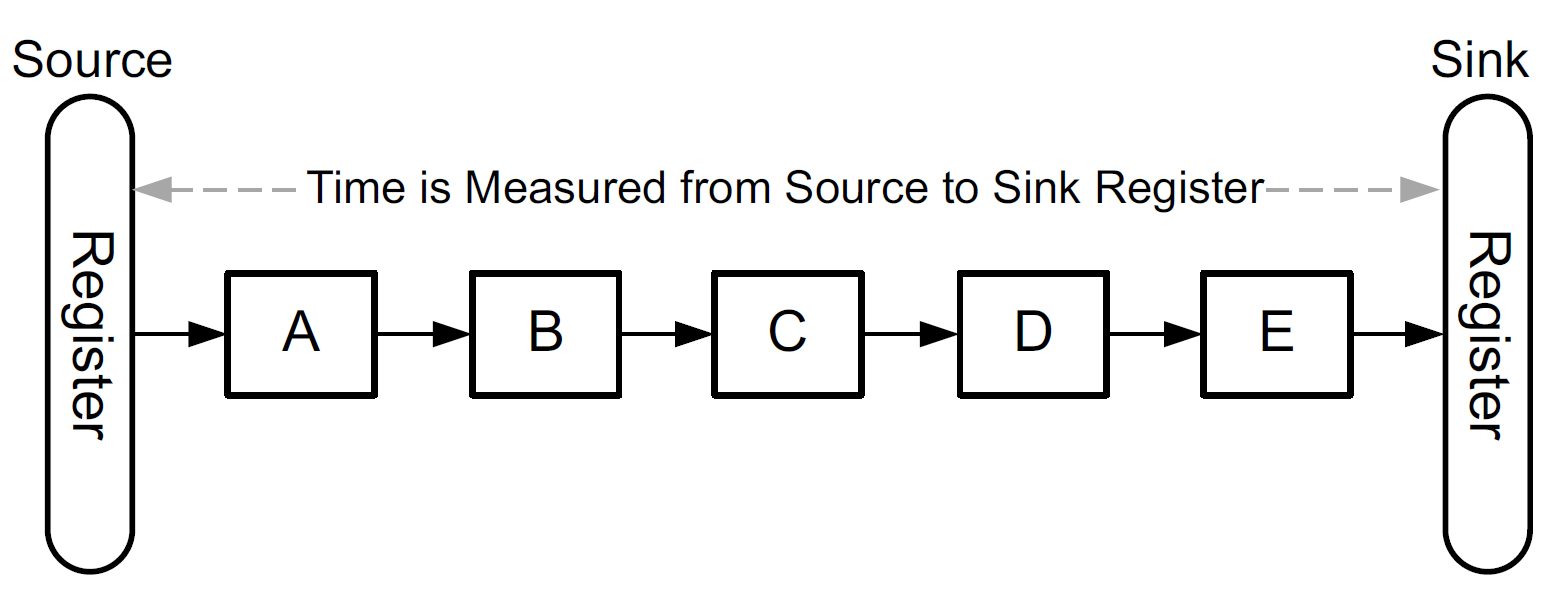
\includegraphics[width=0.6\textwidth]{images/FPGAWOPipe.png}
      \caption{FPGA Implementation without Pipelining}
      \label{FPGAWOPipe}
  \end{center}
\end{figure}

\begin{itemize}
  \item \textbf{Operation timing} in an FPGA is the length of time it takes a signal to travel from a source
  register to a sink register. 
  \item For the case of an FPGA circuit,
  the \textbf{clock frequency} is defined as the longest signal travel time between source and sink
  registers.  
  \item \textbf{Pipelining} in an FPGA is the process of inserting more registers to break up large
  computation blocks into smaller segments. This partitioning of the computation increases
  the latency in absolute number of clock cycles but increases performance by allowing the
  custom circuit to run at a higher clock frequency.
\end{itemize}

\subsubsection{Important points}
\figref{FPGAwithPipe} shows the implementation of the processing architecture in \figref{FPGAWOPipe} after
complete pipelining. Complete pipelining means that a register is inserted between each
building block in the FPGA circuit. 

The addition of registers reduces the timing requirement
of the circuit, which results in a maximum clock frequency. In
addition, by separating the computation into separate register-bounded regions, each
block is allowed to always be busy, which positively impacts the application throughput.

One issue with pipelining is the latency of the circuit. The original circuit of \figref{FPGAWOPipe} has
a latency of one clock cycle at the expense of a low clock frequency. In contrast, the circuit
of \figref{FPGAwithPipe} has a latency of five clock cycles at a higher clock frequency.

\begin{figure}[H]
  \begin{center}
      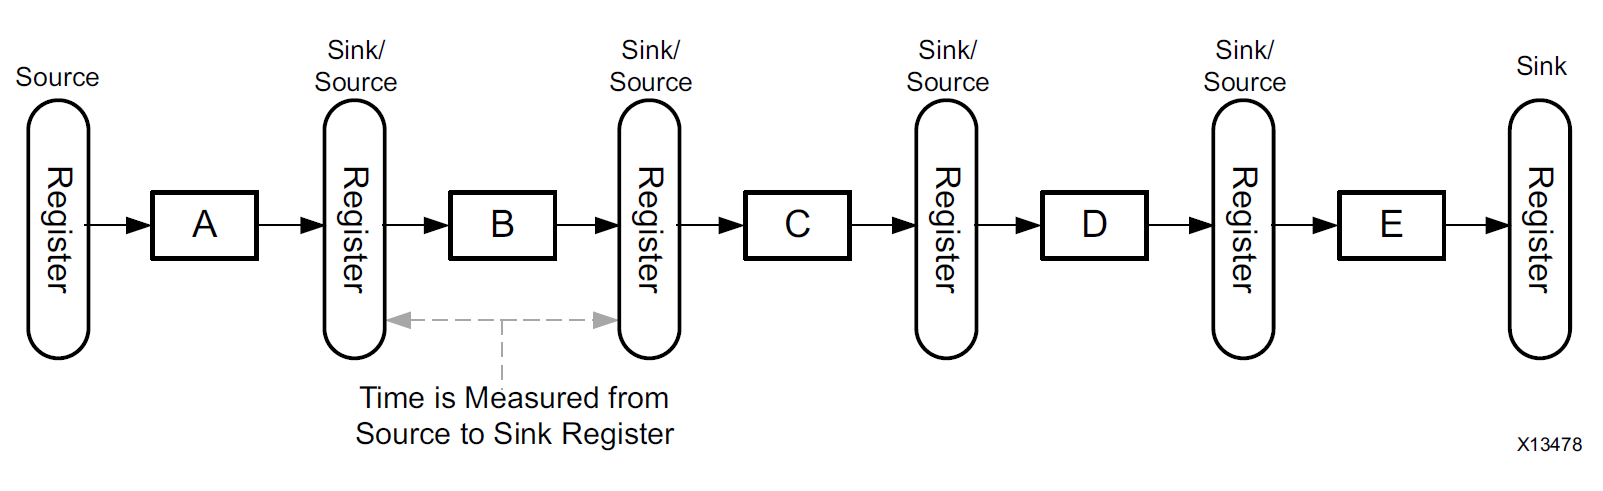
\includegraphics[width=0.8\textwidth]{images/FPGAwithPipe.png}
      \caption{FPGA Implementation with Pipelining}
      \label{FPGAwithPipe}
  \end{center}
\end{figure}

\begin{highlight}
  \textbf{IMPORTANT: The latency caused by pipelining is one of the trade-offs to consider during FPGA design.}
\end{highlight}
\clearpage


\subsection{Throughput}
\textbf{Throughput} is another metric used to determine overall performance of an implementation. It is the number of clock cycles it takes for the processing logic to accept the next input data
sample. With this value, it is important to remember that the clock frequency of the circuit
changes the meaning of the throughput number. 

\par For example, both \figref{FPGAWOPipe} and \figref{FPGAwithPipe} show implementations that require one clock
cycle between input data samples. The key difference is that the implementation in
\figref{FPGAWOPipe} requires 10 ns between input samples, whereas the circuit in \figref{FPGAwithPipe} only
requires 2 ns between input data samples.

\par After the time base is known, it is clear that the
second implementation has higher performance, because it can accept a higher input data
rate.

\begin{highlight}
  Note: The definition of throughput described in this section can also be used when analyzing applications executing on a processor.
\end{highlight}

\subsection{Memory Architecture and Layout}
The memory architecture of the selected implementation platform is one of the physical
elements that can affect the performance of a software application. Memory architecture
determines the upper bound on achievable performance. At some performance point, all
applications on either a processor or an FPGA become memory bound regardless of the
type and number of available computational resources. 


In a processor-based system, the software engineer must fit the application on essentially
the same memory architecture regardless of the specific type of processor. This
commonality simplifies the process of application migration at the expense of performance.
Common memory architecture familiar to software engineers consists of memories that are
slow, medium, or fast based on the number of clock cycles it takes to get the data to the
processor. These memory classifications are defined below.

\begin{table}[H]
  \begin{tabular}{|p{0.15\linewidth} | p{0.80\linewidth}|}
  \hline
  \textbf{Memory Type}    &  \textbf{Definition} \\ \hline
  Slow           & Mass storage devices such as hard drives \\ \hline
  Medium         & DDR memories \\ \hline
  Fast           & On-chip cache memories of different sizes depending on the specific processor \\ \hline
  \end{tabular}
\end{table}

The memory architecture shown in this table assumes that the user is presented with a
single large memory space. Within this memory space, the user allocates and de-allocates
regions to store program data. The physical location of data and how it moves between the
different levels in the hierarchy is handled by the computation platform and is transparent
to the user. In this kind of system, the only way to boost performance is to reuse data in the
cache as much as possible.

\par To achieve this goal, the software engineer must spend large amounts of time looking at
cache traces, restructuring the software algorithm to increase data locality, and managing
memory allocation to minimize the instantaneous memory footprint of the program.

\begin{highlight}
  Although all of these techniques are portable across processors, the results are not. A
  software program must be tuned for each processor it runs on to maximize performance.
\end{highlight}

\par FPGA-based systems can be attached to slow and medium memories
but exhibit the greatest degree of differentiation in terms of available fast memories. That
is, instead of restructuring the software to best use an existing cache, the Vivado HLS
compiler builds a fast memory architecture to best fit the data layout in the algorithm. The
resulting FPGA implementation can have one or more internal banks of different sizes that
can be accessed independently from one another.

\par The use of dynamic memory allocation has long been part of the best practice guidelines for processor-based systems due to the underlying fixed memory architecture.

\par In contrast to this approach, the Vivado HLS compiler builds a memory architecture that is
tailored to the application. This tailored memory architecture is shaped both by the size of
the memory blocks in the program as well as by how the data is used throughout program
execution. Vivado HLS requires that
the memory requirements of an application are fully analyzable at compile time.

\par The benefit of static memory allocation is that Vivado HLS can implement the memory in different ways. Depending on the computation in the algorithm, the Vivado HLS
compiler can implement the memory as registers, shift registers, FIFOs, or BRAMs.

\subsubsection{Registers}
A register implementation of a memory is the fastest possible memory structure. Each independent entity to be stored is embedded into the computation where it is used without the need to address logic or additional delays.

\subsubsection{Shift Register}
In processor programming terms, a shift register can be thought of as a special case of a queue. The key characteristic of a shift register is that every element can be accessed on every clock cycle. In addition, moving all data items to the next adjacent
storage container requires only one clock cycle.

\subsubsection{FIFO}
A FIFO can be thought of as a queue with a single point of entry and a single point of exit. This kind of structure is typically used to transmit data between program loops or functions. There is no addressing logic involved, and the implementation details are completely handled by the Vivado HLS compiler.

\subsubsection{BRAM}
A BRAM is a random-access memory that is embedded into the FPGA fabric. A Xilinx FPGA device includes many of these embedded memories. The exact number of memories is device specific. In processor programming terms, this kind of memory can be thought of as
a cache with the following limitations:

\begin{itemize}
  \item Does not implement cache coherency, collision, and cache miss tracking logic typically found in a processor cache.
  \item Holds its values only as long as the device is powered on (Volatile).
  \item Supports parallel same cycle access to two different memory locations.
\end{itemize}
\clearpage

\section {Vivado High-Level Synthesis}
  The Xilinx Vivado High-Level Synthesis (HLS) compiler provides a programming environment similar to those available for application development on both standard and specialized processors. Vivado HLS shares key technology with processor compilers for the
  interpretation, analysis, and optimization of C/C++ programs. The main difference is in the execution target of the application.
  
  \par By targeting an FPGA as the execution fabric, Vivado HLS enables a software engineer to optimize code for throughout, power, and latency without the need to address the
  performance bottleneck of a single memory space and limited computational resources.
  
  \par Application code targeting the Vivado HLS compiler uses the same categories as any processor compiler. Vivado HLS analyzes all programs in terms of:
  \begin{itemize}
    \item Operations
    \item Conditional statements
    \item Loops
    \item Functions
  \end{itemize}

  
  \begin{highlight}
    IMPORTANT: Vivado HLS can compile almost any C/C++ program. The only coding limitation for Vivado HLS is with dynamic language constructs typical in processors with a single memory space. When using Vivado HLS, the main dynamic constructs to consider are memory allocation and pointers.
  \end{highlight}

                                                    
\subsection{Operations}
Operations refer to both the arithmetic and logical components of an application that are involved in computing a result value. 
\begin{itemize}
  \item With a processor compiler, the fixed processing architecture means that the user can only affect performance by limiting operation dependency and manipulating memory layout to maximize cache performance.
  \item In contrast, Vivado HLS is not constrained by a fixed processing platform and builds an algorithm-specific platform based on user input. This allows an HLS designer to affect application performance in terms of throughput, latency, and power.
\end{itemize} 

\paragraph{Tradeoff between resources, performance, and application}
Although an FPGA does not have a fixed processing architecture, each
device has a maximum number of building blocks it can sustain. Therefore, the designer can evaluate FPGA resources versus application performance versus the number of applications per device.

\subsubsection{Optimizations by vivado HLS}

\begin{itemize}
  \item The scheduling of the operations to reduce the latency is one of the automatic resource optimizations from Vivado HLS.
  \item For memory operations, Vivado HLS analyzes the banks containing the data and where the value is consumed during computation. 
  \item Another way in which Vivado HLS helps the user control the size of the generated circuit is by providing data types for the sizing of variables. Vivado HLS offers the user access to integer, single precision, and double precision data types.
  \item Vivado HLS also offers arbitrary precision data types for eliminating inefficiencies caused due to 32-bit and 64-bit data types.
  \item Arbitrary precision data types reduces the number of resources, the number of levels of logic required to complete an operation, and in the latency of a design.
  \item Based on the size of operations, Vivado HLS automatically does the optimization by pipelining, or division of computation into smaller register-bound regions.
  \item Vivado HLS divides large operators into multiple
  computation stages with a corresponding increase in circuit latency.
\end{itemize}



\subsection{Conditional Statements}
  Conditional statements are program control flow statements that are typically implemented as if, if-else, or case statements. These coding structures are an integral part of most algorithms and are fully supported by all compilers, including HLS. The only difference
  between compilers is how these types of statements are implemented.

  \par With a processor compiler, conditional statements are translated into branch operations that might or might not result in a context switch. The introduction of branches disrupts the maximum instruction execution packing \figref{multiProcessor} by introducing a dependence
  that affects which instruction is fetched next from memory. This uncertainty results in bubbles in the processor execution pipeline and directly affects program performance.

  \par In an FPGA, a conditional statement does not have the same potential impact on  performance as in a processor. Vivado HLS creates all the circuits described by each branch of the conditional statement. Therefore, the runtime execution of a conditional software
  statement involves the selection between two possible results rather than a context switch.


\subsection{Loops}
  Loops are a common programming construct for expressing iterative computation. HLS fully supports loops. The default behavior of HLS is to execute loops in the same schedule as a processor but, HLS can parallelize or pipeline the iterations of a loop to reduce computation latency and increase the input data rate. HLS creates the hardware for the algorithm, it can alter the execution profile of a loop by following optimizations:

  \subsubsection{Optimizations by vivado HLS}
  \begin{enumerate}
    \item To reduce iteration latency, Vivado HLS uses \textbf{Operator Parallelization} to the loop iteration body.
    \item \textbf{Loop Iteration Pipelining} requires user input, as it affects the resource consumption and input data rates of the FPGA implementation.
  \end{enumerate}

  The user controls the level of iteration pipelining by setting the
  \textbf{Loop Initialization Interval (II)}. The II of a loop specifies the number of clock cycles between the start times of consecutive loop iterations. 

  \par To achieve iteration pipelining, HLS analyzes the data dependencies and resource contentions between loop iterations 0 and 1 and automatically resolves issues as follows:
  \begin{itemize}
    \item To resolve data dependencies, HLS alters one of the operations in the loop body or
    queries the user for algorithm changes.
    \item To resolve resource contentions, HLS instantiates more copies of the resource or
    queries the user for algorithm changes.
  \end{itemize}

\subsection{Functions}
  Functions are a programming hierarchy that can contain operators, loops, and other functions. The treatment of functions in both HLS and processor compilers is similar to that
  of loops.

  \par In HLS, the main difference between loops and functions is related to terminology. HLS can parallelize the execution of both loops and functions. To avoid potential confusion when working with HLS, the parallelization
  of function call execution is referred to as \textbf{Dataflow Optimization.}

  The dataflow optimization instructs HLS to create independent hardware modules for all functions at a given level of program hierarchy. These independent hardware modules are capable of concurrent execution and self-synchronize during data transfer.

\subsection{Dynamic Memory Allocation}

Dynamic memory allocation is one of the memory management techniques available in the
C and C++ programming languages. In this method, the user can allocate as much memory
as necessary during program runtime. The size of the allocated memory can vary between
executions of the program and is allocated from a central physical pool of memory. The function calls typically
associated with dynamic memory allocation are shown below:

\begin{table}[H]
  \centering
  \begin{tabular}{|l|l|}
  \hline
  \textbf{C} & \textbf{C++}  \\ \hline
  malloc()   & new()\\ \hline
  calloc()   & delete()\\ \hline
  free()   &  \\ \hline
  \end{tabular}
\end{table} 

As FPGA does not have a fixed memory architecture, HLS synthesizes the memory architecture based on the unique requirements of the
algorithm. Therefore, all code provided to the HLS compiler for implementation in an FPGA
must use compile time analyzable memory allocation only.

\par To aid the user in ensuring that all code provided to HLS is synthesizable, the compiler
executes a coding compliance pass before analyzing the design. This code compliance pass
flags all coding styles that are not suitable for HLS. It is the responsibility of the user to
manually change the code and remove all instances of dynamic memory allocation. 

\begin{highlight}
  Note: HLS cannot synthesize code that includes any of the dynamic memory allocation keywords even if the allocation is constant.
\end{highlight}


\begin{lstlisting}[style=CStyle]
  // Dynamic Memory Allocation in C/C++
  int *A = malloc(10*sizeof(int));
  // This code is not synthesized in HLS.
\end{lstlisting}

There are two possible methods of modifying this code to comply with HLS. 

\paragraph{HLS-Compliant Automatic Memory Allocation}
HLS implements this memory style in strict accordance with the behavior stipulated by C/C++. This means that the memory created to store array A only stores valid data values during the duration of the function call containing this array. Therefore, the function call is
responsible for populating A with valid data before each use.

\paragraph{HLS-Compliant Static Memory Allocation}
The behavior for this type of memory allocation dictates that the contents of array A are valid across
function calls until the program is completely shut down. When working with HLS, the
memory that is implemented for array A contains valid data as long as there is power to the
circuit.

\begin{lstlisting}[style=CStyle]
  // HLS-Compliant Automatic Memory Allocation
  int A[10];

  // HLS-Compliant Static Memory Allocation
  static int A[10];
\end{lstlisting}

Both automatic and static memory allocation techniques can increase the overall software
memory footprint of an algorithm running on a processor.When specifying algorithms in
C/C++ for FPGA implementation, the most important consideration is the overall goal of
the user application. That is, the main goal when compiling to an FPGA is not creating the
best software algorithm implementation. Instead, when using tools like HLS, the goal is to
capture the algorithm in a way that allows the tool to infer the best possible hardware
architecture, which results in the best possible implementation.


\subsection{Pointers}  
A pointer is an address to a location in memory. The HLS compiler supports pointer usage that can be completely
analyzed at compile time. An analyzable pointer usage is usage that can be fully expressed
and computed in a pen and paper computation without the need for runtime information.
  
\begin{lstlisting}[style=CStyle]
  // Valid coding style in which pointers are used to access a
  memory.
  int A[10];
  int *pA;
  pA = A;
\end{lstlisting}      
  

Another supported model for memories and pointers is in accessing external memory.
When using HLS, any pointer access on function parameters implies either a variable or an
external memory. HLS defines an external memory as any memory outside of the scope of
the compiler-generated RTL. This means that the memory might be located in another
function in the FPGA or in part of an off-chip memory, such as DDR.


\clearpage

\section{Software Verification and Vivado HLS}
\subsection{Software Test Bench}
Verification of any HLS-generated module requires a software test bench. The software test
bench serves the following important functions:
\begin{itemize}
    \item To prove that the software targeted for FPGA implementation runs and does not create a segmentation fault.
    \item To prove the functional correctness of the algorithm.
\end{itemize}

\paragraph{Segmentation faults}
Segmentation faults are an issue in HLS as they are in any other compiler. However, there is a difference in how the coding error that caused the issue is detected. 

In a processor-based execution, segmentation faults are caused by a program trying to access a memory location
that is not known to the processor. 
Detection of this error is relatively
straightforward at runtime based on the following sequence of events:
\begin{enumerate}
  \item Processor detects a memory access violation and notifies the operating system (OS).
  \item OS signals the program or process causing the error.
  \item After receiving the error signal from the OS, the program terminates and generates a core dump file for analysis.
\end{enumerate}

\textit{In an HLS-generated implementation, it is difficult to detect a segmentation fault, because
there is no processor and no operating system monitoring program execution.} The only
indicator of a segmentation fault is the appearance of incorrect result values generated by
the circuit. 


\begin{highlight}
  RECOMMENDED: When working with HLS, it is recommended that the designer ensure that the
  software test bench compiles and executes the function without issues on a processor. This guarantees
  that the HLS-generated implementation will not result in a segmentation fault.
\end{highlight}

The other purpose of the software test bench is to prove the functional correctness of an algorithm targeted towards FPGA execution. For the generated hardware implementation,
the HLS compiler guarantees only functional equivalence with the original C/C++ code. Therefore, the existence of a good software test bench is required to minimize efforts in
hardware verification and validation.

A good software test bench is characterized by the execution of thousands or millions of data set tests on the software implementation of an algorithm. This allows the designer to
assert with a high level of confidence that the algorithm was captured properly. However,
even with many test vectors, it is sometimes still possible to detect errors in the
HLS-generated output during hardware verification of an FPGA design. Detecting
functional errors during hardware verification means that the software test bench was
incomplete. Applying the offending test vector to the C/C++ execution reveals the incorrect
statement in the algorithm.

\begin{highlight}
  IMPORTANT: Errors must not be fixed directly in the generated RTL. Any issues with functional
  correctness are a direct result of the functional correctness of the software algorithm.    
\end{highlight}


\begin{highlight}
  TIP: The software test bench used to exercise an algorithm targeted for FPGA implementation with HLS
  does not have any coding style restrictions. The software engineer is free to use any valid C/C++ coding
  style or construct to thoroughly test the functional correctness of an algorithm.    
\end{highlight}


\subsection{Code Coverage}

Code coverage indicates what percentage of the statements in a design are exercised by the
test bench code. This metric, which can be generated by tools like gcov, gives an idea of the
quality of the test vectors used to exercise the algorithm.

\par At a minimum, a test bench must receive a 90\% code coverage score to be considered an adequate test of an algorithm. This means that the test vectors trigger all branches in case statements, conditional if-else statements, and for loops. Aside from the overall coverage
metric, the report generated by code coverage tools provide insight into which parts of a function are executed and which are not.

Running gcov requires that the code is compiled with additional flags that generate the information needed for profiling the execution of a program. Example gcov command on example code named example.c

\begin{lstlisting}[style=CStyle]
  gcc --fprofile-arcs --ftest-coverage example.c
  ./a.out
  gcov example.c    
\end{lstlisting}

\subsection{Uninitialized Variables}
Uninitialized variables are a result of a poor coding style in which the designer does not initialize variables to 0 at the point of declaration. For example, 

\begin{lstlisting}[style=CStyle]
  int A;
  int B;
  ...
  A = B * 100;
\end{lstlisting}

Although some processor compilers resolve the problem by automatically assigning 0 at the point of declaration, HLS does not use this type of solution. HLS assumes that any undefined behavior in the user code can be optimized out of the resulting implementation. This triggers an optimization cascade effect that can reduce the
circuit to nothing. A user can detect this type of error by noticing the empty RTL files for the generated implementation.

\par A better way to detect this type of error is to use code analysis tools, such as \textbf{valgrind \& Coverity}. Both of these tools flag uninitialized variables in the user program. Like all
software quality issues, uninitialized variables must be resolved before the code is compiled with HLS.

\subsection{Out-of-Bounds Memory Access}
In HLS, memory accesses are expressed either as operations on an array or as operations on an external memory through a pointer. In the case of out-of-bounds memory access, the focus is on arrays that are converted into memory blocks by HLS.

\par In a processor compiler, this type of address overflow triggers the address counter to reset to 0.  Although the result is functionally incorrect, this kind of error does not usually result in a program crash.

\par With HLS, accessing an invalid address triggers a series of events that result in an irrecoverable runtime error in the generated circuit. Because the HLS implementation assumes that the software algorithm was properly verified, error recovery logic is not included in the generated FPGA implementation. 

Therefore, an invalid memory address is generated by the implementation of the code to the BRAM resource element. The BRAM then issues an error condition that is not expected by the HLS implementation, and the error is left unattended. The unattended error from the BRAM causes the system to hang and can only be resolved with a device reboot.

\par To catch cases like this before circuit compilation, it is recommended that the tool is executed through a dynamic code checker such as valgrind. Valgrind is a suite of tools designed to check and profile the quality of a C/C++ program. The valgrind Memcheck tool
executes a compiled C/C++ program and monitors all memory operations during execution. This tool flags the following critical issues:
\begin{enumerate}
  \item Use of uninitialized variables
  \item Invalid memory access requests
\end{enumerate}

\begin{highlight}
  RECOMMENDED: Before using HLS to compile a software function for FPGA execution, it is recommended that all of the issues flagged by a dynamic code checker are resolved by the designer.
\end{highlight}



\subsection{Co-Simulation}

Tools for C/C++ program analysis and functionality testing catch most of the issues that affect an HLS implementation. However, these tools are unable to verify whether a sequential C/C++ program maintains functional correctness after parallelization. This issue is resolved in the HLS compiler by the process of co-simulation.

\par Co-simulation is a process in which the generated FPGA implementation is exercised by the
same C/C++ test bench used during software simulation. HLS handles the communication
between the C/C++ test bench and the generated RTL in a manner that is transparent to the
user. As part of this process, HLS invokes a hardware simulator, such as the Vivado simulator,
to emulate how the RTL will function on the device. The main purpose of this simulation is
to check that the parallelization guidance provided by the user did not break the functional
correctness of the algorithm.

\par By default, HLS obeys all algorithm dependencies before parallelization to ensure functional
equivalence with the original C/C++ representation. In cases where an algorithm
dependence cannot be fully analyzed, HLS takes a conservative approach and obeys
dependence. This can lead the compiler to generate a conservative implementation that
does not achieve the target performance goals of the application. 

\par When using co-simulation, it is important to remember that this is a simulation of parallel
hardware being executed on a processor. Therefore, it is approximately 10,000 times slower
than C/C++ simulation. 

\begin{highlight}
  It is also important to remember that the purpose of co-simulation is not to verify the functional correctness of an algorithm. Instead, the purpose is to check that the algorithm was not broken by user guidance to the HLS compiler.
\end{highlight}


\subsection{When C/C++ Verification Is Not Possible}
There are still some cases where the C/C++ representation of an algorithm cannot be fully verified before HLS compilation. 

\par For example, the usage of the
volatile keyword, which is common in device driver development, alerts the compiler
that the pointers are connected to storage elements that might change during the
execution of the function. This kind of pointer must be read or written every time it is
specified in the source code. Traditional compiler optimizations to coalesce pointer
accesses are also turned off by the volatile keyword.

\par The issue with volatile data is that the behavior of the code cannot be fully verified in a
C/C++ simulation. C/C++ simulation does not have the ability to change the value of a
pointer in the middle of the execution of the function under test. Therefore, this type of
code can only be fully verified in an RTL simulation after HLS compilation. The user must
write an RTL test bench to test the generated circuit in all possible cases for each volatile
pointer in the C/C++ source. The use of co-simulation is not applicable in this case, because
it is limited by the test vectors that can be used in a C/C++ simulation.

\clearpage

\section{Design Example: Application Running on a Zynq-7000 SoC}
This design example shows how to take processor code and transform it into an application
that runs on a Zynq-7000 SoC. This example walks through the following steps in the
migration process:

\begin{itemize}
  \item Analyzing and partitioning the processor code
  \item Compiling the program in Vivado HLS
  \item Composing the system in Vivado IP integrator
  \item Connecting processor code and FPGA fabric functions
\end{itemize}

\subsection{Analyzing and partitioning the processor code}
Most software applications targeted for a Zynq-7000 device begin as applications executing on either a standard x86 processor or a DSP processor. Therefore, the first step in migrating a design is to compile the program for the Arm Cortex-A9 processor and analyze its performance. The performance analysis data of a program running on the Arm processor
guides the designer in choosing how to partition the original code between processor and FPGA fabric.

\par Post compilation to the Arm processor, there are two ways of analyzing program performance:
\begin{itemize}
  \item Measuring timing: This method involves instrumenting the code with timers and timing the execution of each sub-function on the processor.
  \item Using code profiling tools: This less intrusive method uses tools, such as gprof, to measure the amount of time spent on a function and to provide statistics on the number of times the function is called.
\end{itemize}

Based on the results of gprof the decision is made where the functions are implemented. After a function is marked for FPGA implementation, the function ports must be analyzed to determine the most suitable hardware interface.


\subsection{Compiling the program in Vivado HLS}

After identifying the functions to run in the FPGA fabric, the designer prepares the source
code for Vivado HLS compilation. 

\begin{highlight}
  RECOMMENDED: When working with multiple projects or modules, it is recommended that the source
  code is separated into different files. This simple technique prevents issues with one module
  compilation affecting the other module in the design.
\end{highlight}

HLS compilation can be controlled using a Tool Command Language (Tcl) script file. A Tcl
script file, which is analogous to a compilation Makefile, instructs the compiler which
function to implement and FPGA device to target. The script is divided into the following sections:

\begin{description}
  \item[Project setup] This section includes the source files and the name of the function to be compiled.
  Guiding the Vivado HLS compiler is an iterative process of applying directives or
  pragmas to the design source code. Each successive refinement of a design is called a
  solution. All projects have at least one solution.
  \item[Solution setup] This section establishes the clock frequency and device for which the software function
  is compiled. If the designer is guiding the compiler through the use of directives, the
  solution directives are included in this section of the script.
  \item[Compilation setup] This section drives the RTL generation and packaging. The assembly of HLS programs
  into an FPGA device application requires the use of the Vivado IP
  integrator, which is a system composition tool. IP integrator requires modules to be
  packed in the equivalent of a software object file.
\end{description}

Interface pragmas define how the module is connected in the FPGA fabric. The definition
process is separated into interface behavior and interface mapping.

\subsection{Composing the system in Vivado IP integrator}
Vivado IP integrator is a Xilinx FPGA design tool for system composition. One use of this
tool is to take the blocks generated by the HLS compiler and connect them into the
processing platform that executes the user application. In software development terms, IP
integrator is analogous to a linker that combines all program objects into a single bitstream.
A bitstream is the binary file used to program the FPGA fabric.

\subsection{Connecting processor code and FPGA fabric functions}
After the FPGA fabric programming binary is created in IP integrator, the designer must
create the software that runs on the processor. The purpose of this software is to initialize
the FPGA fabric functions, launch execution, and receive results from the fabric. For the
overall application to be functionally equivalent to the original processor code, each
function running in the FPGA fabric requires the following functionality in the code running
on the Arm Cortex-A9 processor:

\begin{itemize}
  \item Address mapping
  \item Initialization
  \item Start function
  \item Interrupt service routine (ISR)
  \item Interrupt registration in the processor exception table
  \item New main function to run the system
\end{itemize}

\clearpage

\section{Verification of a Complete Application}

In FPGA design, a complete application refers to a hardware system that implements the
functionality captured by the software representation of a design. There are two main
categories of systems that can be built on an FPGA using the Vivado HLS compiler:
\begin{enumerate}                                      
  \item Standalone Compute Systems                                   
  \item Processor-Based Systems
\end{enumerate}

\subsection{Standalone compute systems}
The standalone compute system is an FPGA implementation created by one or more
HLS-generated modules connected together to implement a software application. In these
types of systems, the configuration of the algorithm is fixed and loaded during device
configuration. The modules generated by the HLS compiler are connected to external FPGA
pins for data transmit and receive transactions. This is the easiest kind of system to verify.
The verification of a standalone system is divided into the following stages:
\begin{enumerate}
  \item Module verification
  \item Connectivity verification
  \item Application verification
  \item Device validation
\end{enumerate}

\subsubsection{Module Verification}
Module verification of an HLS-generated block is covered in section "Software
Verification and Vivado HLS". After the block is fully verified for functional correctness in
both software and co-simulation, the designer must test the block for in system error
tolerance.

\par Both software simulation and co-simulation are focused on testing the functional
correctness of an algorithm in isolation. That is, the algorithm and compiled module are
tested to ensure correct functionality when all inputs and outputs are handled in an ideal
manner. This thorough level of testing helps to ensure correctness after data is supplied to
the module. It also helps to reduce the verification burden of later stages by eliminating the
internal processing core of a module as a possible source of error. \textbf{The only module-level
issue that is not handled by this methodology is verification that the module can recover
fully from incorrect handshaking at its interfaces.}

\par In-system testing tests how the HLS-generated module reacts to incorrect toggling of its
input and output ports. The purpose of this testing is to eliminate I/O behavior as an error
source that can crash or otherwise adversely affect the module under test. The types of
improper use cases tested in this methodology are:

\begin{itemize}
  \item Erratic clock signal toggling
  \item Reset operation and random reset pulsing
  \item Input ports receiving data at different rates
  \item Output ports being sampled at different rates
  \item Interface protocol violations
\end{itemize}

These tests, which are examples of system-level behavior, ensure that the HLS-generated
module functions as expected under all circumstances. The amount of testing required at
this stage depends on the types of interfaces and the integration methodology. By using
HLS default settings to generate AXI-compliant interfaces, the designer can avoid writing
an exhaustive test bench of incorrect system-level behavior. AXI-compliant interfaces are
fully tested and verified by the developers of the HLS compiler.


\subsubsection{Connectivity Verification}
Connectivity verification is a sequence of tests to check that the modules in an application
are properly connected to each other. As with module verification, the amount of testing
required depends on the system integration methodology. FPGA design tool assistance is provided in both the Xilinx System Generator and Vivado IP
integrator design flows. These graphical module connection tools handle all the aspects
related to module connection. 

\par The manual integration flow requires the user to write an application top-level module in
RTL and manually connect the RTL ports of every module that makes up an application. This
is the most error-prone flow and must be verified. The amount of testing required can be
decreased by using HLS compiler defaults and generating AXI interfaces for every module
port.

\par For systems built around AXI interfaces, the connectivity can be verified through the use of
a bus functional model (BFM). The BFM provides the Xilinx-verified behavior of AXI buses
and point-to-point connections. These models can be used for traffic generators, which
help prove the correct connection of HLS-generated modules as part of an RTL simulation.

\begin{highlight}
  IMPORTANT: It is important to remember that the purpose of this simulation is only to check
  connectivity and the proper flow of data through the system. The connectivity verification step does not
  verify the functional correctness of the application.  
\end{highlight}

\subsubsection{Application Verification}
Application verification is the final step before running the application on the FPGA device.
Application verification focuses on checking that the original software model matches the
results of the FPGA implementation. If the application is composed of a single
HLS-generated module, this stage is the same as module verification. In cases where the
application is composed of two or more HLS-generated modules, the verification process
starts with the original software model.
The designer must extract application input and output test vectors from the software
model to be used in an RTL simulation. Because the construction of the hardware
implementation is verified in multiple stages, the application verification does not need to
be an exhaustive simulation. The simulation can run as many test vectors as needed for the
designer to feel confident in the FPGA implementation.

\subsubsection{Device Validation}
After an application is assembled in RTL using either automated or manual integration
flows, the design goes through an additional compilation stage to generate the binary or
bitstream required to program the FPGA. In the terminology of FPGA design, the
compilation of RTL into a bitstream is referred to as logic synthesis, implementation, and
bitstream generation. Once the bitstream is generated, the FPGA device can be
programmed. The application is validated after the hardware runs correctly for an amount
of time specified by the designer.
\clearpage

\subsection{Processor-based systems}
For the module and connectivity verification stages, the verification flow for a
processor-based system is the same as the standalone system. The major difference is that
a portion of the application is running on the processor. 

This partitioning presents a verification
challenge that can be addressed through the use of the following technologies:
\begin{itemize}
  \item Hardware in the loop (HIL) verification
  \item Virtual platform (VP) verification
\end{itemize}

\subsubsection{Hardware in the Loop (HIL) Verification}
HIL verification is a verification methodology in which the simulation of part of the system
under test is executed in the FPGA fabric. The main advantages of HIL verification versus verification are:
\begin{itemize}
  \item No simulation inconsistencies between a processor model and the actual processor
  \item Code running on the processor is executed at the speed of the FPGA device
  \item Full visibility into how each generated module operates through RTL simulation
\end{itemize}

When using HIL verification, it is important to remember the performance characteristics of
this technology. Although the processor code runs in the actual hardware, the FPGA fabric
is fully simulated on the designer’s workstation. HIL verification is
only recommended for verifying the major interactions between the processor and the
FPGA fabric, not every use case in the application. The key application behaviors to check
with HIL verification are:
\begin{itemize}
  \item Vivado HLS driver integration into the processor code
  \item Writing configuration parameters from the PS to the PL
  \item Interrupt from the PL to the PS
\end{itemize}


\subsubsection{Virtual Platform(VP) Verification}
Virtual platform technology is an established method of overlapping software and
hardware development. A virtual platform is a
software simulation of both the application and the hardware platform on which it runs. The
models used for the PL portion of the design can be in C, C++, SystemC, or RTL. This
simulation platform can be used as a proxy for the other recommended verification stages
with varying degrees of fidelity to the hardware implementation.

\par In the fastest use case of the virtual platform, the application modules targeted to the PL
are simulated from the C/C++ source code provided to the Vivado HLS compiler. This setup
results in a functionally correct simulation that allows the designer to test the algorithm for
correct computation. As modules are optimized and compiled with Vivado HLS, the
generated RTL can replace the software version of the module to enable connectivity
testing and timing driver simulation.

\begin{highlight}
  IMPORTANT: It is important to remember that adding RTL modules impacts the runtime on the virtual
  platform and slows down execution.  
\end{highlight}


\subsubsection{Device Validation}
The purpose of device validation is to check all the application use cases in which the
processor interacts with the FPGA fabric. As in the case of standalone execution, this
process involves running the complete application for a certain amount of time on the FPGA/SoC.
The purpose of this test is to check all the application corner cases with
regard to the interaction between the PS and PL portions of the design.


\iffalse

Chapter 5: Computation-Centric Algorithms
  Overview                                                     
  Data Rate Optimization    

Chapter 6: Control-Centric Algorithms
  Overview                                                     
  Expressing Control in C/C++                                  
  UDP Packet Processing    

\fi